\documentclass[letterpaper,11pt,oneside]{article}
\usepackage[left=0.75in, right=0.5in, bottom=1.25in, top=0.4in]{geometry}
\usepackage{graphicx}
\graphicspath{ {/}}

\begin{document}
	\begin{center}
		\textbf{{\huge SOUJANYA AVADHANI M D}}\\
	\end{center}
	\vspace{-2ex}
	\noindent\hrulefill
	\vspace{5ex}
	
	\noindent{\large  {\#9 KT-45, Vijay Apartments, \#103,}} \hfill \large {Contact: 8277399387}
	\\
	\large {16th cross, between 8th and 6th main,} \hfill \large {E-mail id: soujanyaavadhani@gmail.com}
	\\
	\large {Malleswarm, Bangalore, 560-055,}
	\\
	\large {Karnataka.}
    
    \hfill 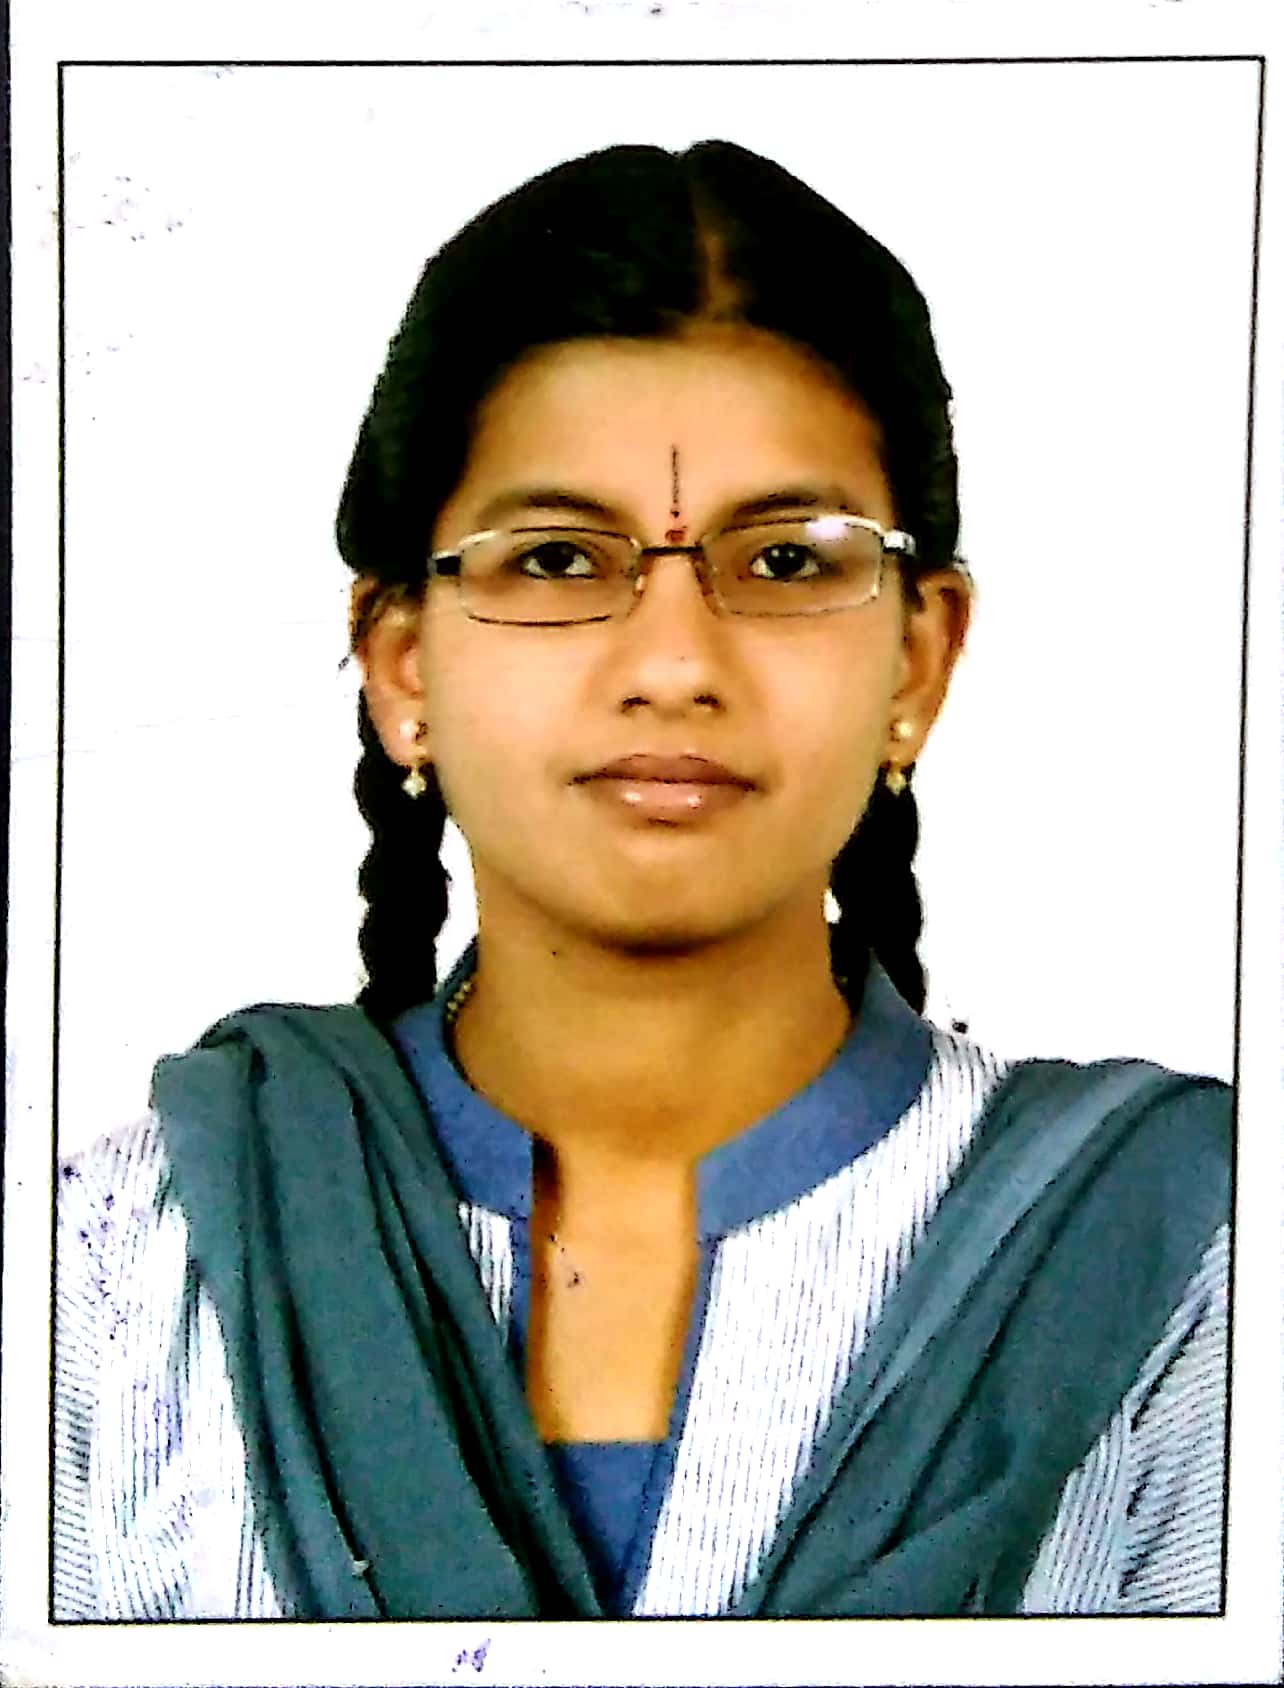
\includegraphics[scale=0.1]{SOUJANYA_AVADHANI_M_D.jpg}\\	
    
    \noindent{\textbf{\underline{\Large CAREER OBJECTIVE:}}}\\
    \\
    \noindent{\large To work with an organisation where I can effectively utilize and contribute my skills and ideas towards the organisation's goals and develop my career.}\\
    \\
    \\
    \noindent{\textbf{\underline{\Large EDUCATION:}}}\\
    \\
    \begin{tabular}{ |c|c|c|c|c| } 
    	\hline
    	\Large{\textbf{Qualification}} & \Large{\textbf{Year of}} & \Large{\textbf{Institution}} & \Large{\textbf{University}} & \Large{\textbf{Percentage}} \\
    	& \Large{\textbf{completion}} & & & \Large{\textbf{of marks}} \\
    	\hline
    	
    	B.E. & 2020 & R.V. College & Autonomous & 9.72 \\
    	(Elecrtonics and & (pursuing) & of Engineering & -Affiliated & (CGPA - 3\\
    	Communication) & & & to VTU & semesters) \\
    	\hline
    	
    	& & Vidya Mandir & Karnataka & \\
    	P.U.C. & 2016 & Independent & State Board &  98.16\% \\
    	&  & P.U. College & & \\
    	
    	\hline
    	& & Sri Vidya Mandir & &\\
    	S.S.L.C. & 2014 & Education & KSEEB & 98.72\% \\
    	& & Society & & \\
    	
    	\hline
    \end{tabular}
    
    \vspace{2ex}
    \pagebreak
    
    \textbf{\underline{\Large PROJECTS:}} \begin{enumerate}
    	\item 
    	\textbf{\underline{\Large Planter Bot (December, 2017 to March, 2018):}}\\
    	\\
    	This project was undertaken as a part of E-Yantra Robotics Competition - 2017, IIT Bombay.
    	
    	\vspace{2ex}
    	
    	\textbf{\large Project Objective:} 
    	\begin{enumerate}
    		\item To traverse different zones in the given arena with the help of image processing.
    		\item To overlay the corresponding 'seedling images' on 'plantation backgroungd' image depending on the number of 'colour markers' detected.\\ 
    	\end{enumerate}
    	\textbf{\large Roles and Responsibilities:}\\
    	\\
    	Contributed to building the chassis and algorithm of the project.\\
    	\\
    	\textbf{\large Challenges:} 
    	\begin{enumerate}
    		\item Image Processing
    		\item Shadow and Glare Removal
    		\item Path and Zone Differentiation
    		\item Switching algorithms for following black and white paths
    		\item Image Overlay
    	\end{enumerate}
    	
    	\vspace{2ex}
    	
    	\item 
    	\textbf{\underline{\Large Greenhouse Monitering System(September, 2017 to November, 2017):}}\\
    	\\
    	This project was undertaken for self-study during third semester.
    	
    	\vspace{2ex}
    	
    	\textbf{\large Project Objective:}
    	\begin{enumerate}
    		\item To moniter a greenhouse remotely with the aid of IoT technology.
    		\item To automatically regulate the temperature, humidity, soil moisture conditions within the greenhouse.\\
    	\end{enumerate}
    	\textbf{\large Roles and Responsibilities:}\\
    	\\
    	Contributed to algorithm amd code of the project. Also designed a prototype of the greenhouse.\\
    	\\
    	\textbf{\large Challenges:}
    	\begin{enumerate}
    		\item Interfacing a LCD Display to Raspberry-Pi
    		\item Interfacing the temperature - humidity sensor, ldr and soil moisture sensors
    		\item Effectively reading the input data from the sensors
    		\item uploading the read values to a local cloud 
    		\item setting thresholds to switch on the regulatory systems
    	\end{enumerate}
    	
    	\vspace{2ex}
    	
    	\textbf{\underline{\Large Grid Solver Bot(May, 2017 to June, 2017):}}\\
    	\\
    	This project was undertaken to exhibit during Srushti Exhibition - 2017.
    	
    	\vspace{2ex}
    	
    	\textbf{\large Project Objective:}\\
    	\\
    	To build a robot which traverses to a partical location upon specifying the x,y co-ordinates of the location.\\
    	\\
    	\textbf{\large Roles and Responsibilities:}\\
    	\\
    	Contributed to algorithm amd code of the project.\\
    	\\
    	\textbf{\large Challenges:}
    	\begin{enumerate}
    		\item To interface IR sensors to arduino
    		\item To write efficient path traversing and direction alignment algorithm to take the shortest path to reach the specified location 
    		\item To make the bot bluetooth controlled
    	\end{enumerate}
    	\end{enumerate}
\end{document}	